\lecture{Лекция 2}{lec2}
\subtitle{Лекция 2 --- Информация и кодирование}
\frame[plain]
{\titlepage}	% Титульный слайд

\section{Информация и кодирование}
\section{Информация}
 \subsection{Информация}
\begin{frame}
\frametitle{Основные определения}


\begin{block}{Информация}
  Информация (от лат. informatio) — отражение реального (материального) мира, выраженное в виде сигналов и знаков.

\end{block}

\pause

\begin{block}{Информатика}
Изучает способы хранения, обработки, передачи, классификации, визуализации и т.п. информации.
\end{block}
\pause
\begin{block}{Информация и ее представление}
Различают
 \begin{itemize}
 \item{представление или изображение информации (внешняя форма);}
 \item{значение (абстрактная информация)}
 \item{отношение к реальному миру (связь абстрактной информации с действительностью)}
 \end{itemize}
 
\end{block}

\end{frame}

\begin{frame}
\frametitle{Основные определения}
\begin{block}{Информационная технология}
Конкретный способ хранения, обработки, передачи, классификации, визуализации и т.п. информации.
\end{block}
\pause
\begin{block}{Виды информационных технологий}
\begin{itemize}
	\item Обработка текста
	\item Обработка графики
	\item СУБД
	\item Обработка больших данных
	\item и др.
\end{itemize}
\end{block}

\end{frame}

\begin{frame}[fragile,squeeze]{Данные, информация, знания}

\begin{block}{Сигнал, сообщение}
 Это физический уровень информации. Например сигнал светофора или звуковые колебания.
\end{block}
\pause
\begin{block}{Данные}
 Дискретные или аналоговые сигналы, которые может обработать компьютер.
\end{block}
\pause
\begin{block}{Знания}
 Большие массивы данных объединенные сложной внутренней структурой. 
\end{block}
\end{frame}

\begin{frame}[fragile,squeeze]{Данные, информация, знания}

\begin{block}{Свойства информации}
 \begin{itemize}
	 \item абстрактность
	 \item неотделимость от носителя
 \end{itemize}
 \end{block}

\end{frame}

 \subsection{Информационный процесс}
\begin{frame}[fragile,squeeze]{Информационный процесс}


\begin{block}{Информационный процесс}
 Информационный процесс описывает посдедовательность действий, выполняемых с информацией или данными.
 Система, реализующая информационный процесс, называется информационной системой.
 \end{block}
\begin{block}{Виды информационных процессов}
 \begin{itemize}
	 \item передача информации
	 \item хранение информации
	 \item обработка информации
	 \item восприятие (распознавание) информации
 \end{itemize}
 \end{block}
\end{frame}


\section{Кодирование и измерение информации}
\subsection{Основы комбинаторики}
\begin{frame}
\frametitle{Комбинаторика}
Комбинаторика --- раздел математики, который изучает задачи выбора и расположения элементов из некоторого основного множества в соответствии с заданными правилами. 

Формулы и  принципы  комбинаторики  используются  в  теории информации для расчета количества информации, в теории вероятности, статистике и в других науках. 

Мы будем рассматривать комбинаторные формулы на множествах содержащих только не повторяющиеся элементы.
\end{frame}


\begin{frame}
\frametitle{Правила суммы и произведения}
{\bf Правило суммы.} Если элемент $a$ можно выбрать $m$ способами, а элемент
$b$ - $n$ способами, причём любой выбор элемента $a$ отличен от любого выбора
элемента $b$, то выбор <<$a$ или $b$>>$\;$ можно сделать

$m+n$ способами.

\pause

{\bf Правило произведения.} Если элемент $a$ можно выбрать $m$ способами, а элемент
$b$ - $n$ способами, то выбор пары элементов <<$a$ и $b$>>$\;$ можно сделать

 $m\cdot n$ способами.
\end{frame}

\begin{frame}
\frametitle{Правила суммы и произведения}
\framesubtitle{Примеры}
\textbf{Задача:} Монету бросают трижды. Сколько разных последовательностей орлов и решек можно при этом получить?
\pause
\textbf{Решение}

В каждом броске есть 2 варианта, соответственно получаем

$$ \underline{2}\cdot \underline{2} \cdot \underline{2} = 8 $$


\end{frame}

\begin{frame}
\frametitle{Правила суммы и произведения}
\framesubtitle{Примеры}
\textbf{Задача:} Cколько существует различных семизначных телефонных номеров (cчитается, что номер начинаться с нуля не может)? 
\pause
\textbf{Решение}

Первую цифру можно выбрать 9 способами, а каждую из шести остальных – 10 способами. Итого, $9\cdot10^6$ способов

\end{frame}

\begin{frame}
\frametitle{Перестановки}
{\bf Перестановки} Числом перестановок без повторений из $n$ элементов называется количество способов выписать в строчку все эти $n$ элементов. 

Оно обозначается $P_n$ и находится по формуле $P_n=n!$.

$$ n! = n\cdot(n-1)\cdots 1$$

\end{frame}



\begin{frame}
\frametitle{Перестановки}
\framesubtitle{Примеры}
\textbf{Задача:} Сколько существует трёхзначных чисел, в записи которых цифры 1, 2, 3 встречаются ровно по одному разу?
\pause
\textbf{Решение}

На первое место можно поставить любую из трёх цифр, на второе --- любую из двух оставшихся, а на третье --- последнюю оставшуюся цифру. Таким образом, всего получается 6 чисел.

$$3! = 6$$  чисел. 

\end{frame}

\begin{frame}
\frametitle{Перестановки}
\framesubtitle{Примеры}
\textbf{Задача:} 
а) Сколькими способами 28 учеников могут выстроиться в очередь в столовую?\\
б) Как изменится это число, если Петю Иванова и Колю Васина нельзя ставить друг за другом? 
\pause
\textbf{Решение}

a) $28!$

б) Временно уберём из очереди Колю. Оставшихся учеников можно расставить 27! способами. Колю в каждую очередь можно вставить 28 способами, но два из них – перед Петей и после него – запрещены. \\
$26\cdot27!$

\end{frame}

\begin{frame}
\frametitle{Размещения}
{\bf Размещения} Числом размещений  из $n$ элементов по $k$ называется количество способов выписать в строку $k$ различных элементов, каждый из которых выбран из данных $n$ (элементы могут повторяться, сточки отличающиеся порядком, считаются разными). Оно обозначается $A_n^k$ и находится
по формуле

$$A_n^k=\frac{n!}{(n-k)!}$$
\end{frame}



\begin{frame}
\frametitle{Размещения}
\framesubtitle{Примеры}
\textbf{Задача:} Сколько существует различных последо-вательностей из символов "A", "B", "C", "D" и "E" длиной ровно 3 символа? (При условии, что символы не могут повторяться.)

\pause
\textbf{Решение}

Необходимо определить количество размещений $n = 5$ элементов (символы <<A>>, <<B>>, <<C>>, <<D>> и <<E>>) в группах по $m = 3$ элемента (длина цепочек символов). Для этого воспользуемся формулой:

$$A_5^3=\frac{n!}{(n-k)!}=\frac{5!}{(5-3)!}=\frac{5!}{2!}=3\cdot4\cdot5=60$$

\end{frame}

\begin{frame}
\frametitle{Сочетания}
{\bf Сочетания.} Числом сочетаний из $n$ 
элементов по $k$ называется количество способов выбрать $k$ элементов из данных
$n$ различных элементов (наборы, отличающиеся лишь порядком, считаются
одинаковыми). 

Оно обозначается $C_n^k$ и находится по формуле

$$C_n^k=\frac{A_n^k}{P_k}=\frac{n!}{k!(n-k)!}$$.


\end{frame}



\begin{frame}
\frametitle{Сочетания}
\framesubtitle{Примеры}
\textbf{Задача:} Пульт управления состоит из 9 переключателей, каждый из которых может пребывать в одном из двух состояний: <<включён>> или <<выключен>>. Сколько различных режимов работы оборудования может обеспечить данный пульт, если одновременно могут быть включены только любые четыре переключателя? \\
\textbf{Решение}
Необходимо определить количество возможных сочетаний $n = 9$ элементов (общее количество выключателей) в группах по $m = 4$ элемента (выключателя). При этом порядок их включения не важен.

$$С_9^4=\frac{9!}{4!(9-4)!}=\frac{9!}{4!5!}=\frac{6\cdot 7\cdot 8\cdot 9}{2\cdot 3\cdot 4}=126$$

\end{frame}

 \subsection{Дискретный и аналоговый сигнал}

\begin{frame}[fragile,squeeze]{Дискретный и аналоговый сигнал}
\begin{block}{Аналоговый сигнал}
 сигнал, у которого каждый из представляющих параметров описывается функцией времени и непрерывным множеством возможных значений (звук, свет, электрический ток).
\end{block}
\pause
\begin{block}{Дискретный сигнал}
сигнал, который является прерывистым (в отличие от аналогового) и который изменяется во времени и принимает любое значение из списка возможных значений. Список возможных значений может быть непрерывным или квантованным. 
\end{block}
\pause
\begin{block}{Цифровой сигнал}
 сигнал, который можно представить в виде последовательности дискретных (цифровых) значений. В наше время наиболее распространены двоичные цифровые сигналы
\end{block}

\end{frame}

\begin{frame}[fragile,squeeze]{Дискретный и аналоговый сигнал}
Аналоговый сигнал
 \includegraphics[height=2cm]{images/analog.png}
\pause
Дискретный сигнал
 \includegraphics[height=2cm]{images/discrete.png}

\pause
Цифровой сигнал
  \includegraphics[height=2cm]{images/digital.png}


\end{frame}

 \subsection{Понятие кода}
\begin{frame}[fragile,squeeze]{Кодирование информации}
\begin{block}{Код}
 Система правил переводящая символы одного алфавита в символы другого алфавита.
\end{block}
\pause
\begin{block}{Кодирование и декодирование}
 Перевод сообщения из одного алфавита в другой.
 Декодирование --- обратная операция.
\end{block}
\pause
\begin{block}{Кодер и декодер}
 Устройства выполняющие кодирование и декодирование.
\end{block}

Приведите пример незакодированного сообщения
\end{frame}

 \begin{frame}[fragile,squeeze]{Подходы к измерению информации}

 \begin{itemize}
	

\item АЛФАВИТНЫЙ --- основан на подсчете числа символов в сообщении. Этот подход не связывает количество информации с содержанием сообщения, позволяет реализовать передачу, хранение и обработку информации с помощью технических устройств, не теряя при этом содержания (смысла) сообщения.
\pause
\item ВЕРОЯТНОСТНЫЙ --- Согласно Шеннону, количество информации в сообщении характеризуется уменьшением неопределенности какой-либо ситуации после получения сообщения. \\
По Шеннону, информация --- уменьшение неопределенности наших знаний.
 \end{itemize}

\end{frame}
 \subsection{Алфавитный подход}
\begin{frame}[fragile,squeeze]{Алфавит и язык}

 Для сообщений, которыми обмениваются люди, в большинстве случаев имеются соглашения относительно их формы.
О таких сообщениях мы говорим, что они передаются в языковой форме, что они составлены на некотором языке. При этом слово \alert{язык} используется в существенно более широком смысле, чем в случае связанного с ним понятия <<говорить>>. 

Мы знаем разговорный и письменный языки, язык глухонемых, построенный на жестах и мимике, печать для слепых
воспринимаемую осязанием и др.

\pause
\begin{block}{Алфавит}
 Набор знаков для изображения элементов языка. Алфавиты бывают конечные и бесконечные. Конечный алфавит является дискретным. Знаки в алфавите не повторяются.
\end{block}


\end{frame}


\begin{frame}[fragile,squeeze]
\frametitle{Алфавит и язык}
\framesubtitle{ Виды языков}

\begin{itemize}
	\item естественные \\создаются условно случайным образом на основе коммуникации между людьми);\pause
	\item искусственные;\\ создаются для специальных целей либо для определенных групп людей: язык математики, морской семафор, язык программирования и т.п.;\pause
	\item формальные\\характеризуются точными правилами построения выражений и их понимания, обеспечивая непротиворечивое, точное и компактное отображение свойств и отношений изучаемой предметной области (моделируемых объектов): язык логики, язык программирования.
\end{itemize}

\end{frame}

\begin{frame}[fragile,squeeze]
\frametitle{Единицы информации}

Количество символов (знаков) языка всегда конечно и называется \alert{Мощностью алфавита}.

Наименьшим пригодным для кодирования информации алфавитом является алфавит, состоящий из двух символов. Каждый из этих символов будет являться наименьшей единицей информации.
\pause

Чтобы осуществить кодирование, достаточно двух символов: 0 или 1  составляет 1 бит  ( bit )

BInary digiT --- (двоичный знак)
\end{frame}

\begin{frame}[fragile,squeeze]
\frametitle{Единицы информации}

1 байт  =  8 бит\\\pause
1 Кбайт  =  1024 байт  =  $2^{10}$ байт\\\pause
1 Мбайт  =  1024 Кбайт  =  $2^{20}$ байт\\\pause
1 Гбайт  =  1024 Мбайт  =  $2^{30}$ байт\\\pause
1 Тбайт  =  1024 Гбайт  =  $2^{40}$ байт\\\pause
1 Пбайт  =  1024 Тбайт  =  $2^{50}$ байт\\\pause
1 Эбайт  =  1024 Пбайт  =  $2^{60}$ байт\\\pause
1 Збайт  =  1024 Эбайт  =  $2^{70}$ байт\\\pause
1 Йбайт  =  1024 Збайт  =  $2^{80}$ байт\\

\end{frame}

\begin{frame}[fragile,squeeze]
\frametitle{Способы кодирования}

\textbf{Двоичное равномерное кодирование} --- каждый символ кодируется одинаковым количеством бит.

\pause
\textbf{Двоичное неравномерное кодирование} --- количество бит, использующихся для кодирования символов, различается.

\end{frame}

 \subsection{Равномерное кодирование}
\begin{frame}[fragile,squeeze]
\frametitle{Равномерное кодирование}

Код называется равномерным (или кодом постоянной длины), если все его кодовые слова содержат одинаковое число букв (одинаковую длину слов).

Для кодирования одного символа алфавита мощности $N$ потребуется минимальное количество бит $i$, равное наименьшему  показателю степени числа 2, при котором значение степени больше либо равно N. \\
Формула Хартли

$$i = log_2N.$$

При этом результат следует округлить до большего целого.

\end{frame}
\begin{frame}[fragile,squeeze]
\frametitle{Равномерное кодирование}
\framesubtitle{Пример}

\textbf{Задача:} Компьютерная игра состоит из 20 уровней, на каждом из которых игроку нужно отыскать 6 секретных ключей. При переходе с уровня на уровень у игрока остаются все найденные ключи. Какое минимальное количество бит потребуется для кодирования номеров секретных ключей?  \\ \pause
\textbf{Решение}
Определим количество ключей:	$20\cdot 6  =  120$

Таким образом, требуется закодировать 120 различных состояний в двоичной системе. 
$$i  = log_2120  =  7.$$

\end{frame}


 \subsection{Неравномерное кодирование}
\begin{frame}[fragile,squeeze]
\frametitle{Неравномерное кодирование}
Для однозначного декодирования неравномерного двоичного кода требуется выполнение условий Фано (Fano conditional):
\begin{itemize}
	\item Ни одно кодовое слово не является началом другого кодового слова (прямое условие)
\item Ни одно кодовое слово не является концом другого кодового слова (обратное условие)
\end{itemize}

Такие коды называются префиксными

\end{frame}
\begin{frame}[fragile,squeeze]
\frametitle{Неравномерное кодирование}
\framesubtitle{Пример}

Префиксный код легче всего представить в виде двоичного дерева, в котором  листы помечены  символами, которые объединяются для формирования сообщения. 

Кодировка символа определяется по пути вниз от корня дерева к листу, который содержит этот символ: 
бит 0 ---левая ветвь, бит 1 правая ветвь. В следующем дереве серые квадраты являются листами (внешними узлами). 

\end{frame}

\begin{frame}[fragile,squeeze]
\frametitle{Неравномерное кодирование}
\framesubtitle{Пример}

Префиксный код легче всего представить в виде двоичного дерева, в котором  листы помечены  символами, которые объединяются для формирования сообщения. 

\begin{tabular}{cc}

\raisebox{-0.5\height}{\includegraphics[height=4cm]{images/prefix.png}} \pause & %
\begin{tabular}{|c|c|}
\hline 
Символ & Код\tabularnewline
\hline 
a & 0\tabularnewline
\hline 
b & 111\tabularnewline
\hline 
c & 1011\tabularnewline
\hline 
d & 1010\tabularnewline
\hline 
r & 110\tabularnewline
\hline 
! & 100\tabularnewline
\hline 
\end{tabular}\tabularnewline

\end{tabular}

\end{frame}

 \subsection{Вероятностный подход}

 \begin{frame}[fragile,squeeze]
\frametitle{Вероятность}

Вероятность $(0 \leq р \leq 1)$ – количественная оценка возможности наступления какоголибо события.

В качестве события можно рассматривать исход некоего опыта. 
Множество всех возможных исходов некоторого опыта составляют полную группу событий. 

Сумма вероятностей всех возможных исходов равна 1. 

События, наступающие с одинаковой долей вероят-ности называются равновероятными.

Если есть N разных равновероятных событий, то вероятность наступления одного из них $p = \frac{1}{N}$

\end{frame}

\begin{frame}[fragile,squeeze]
\frametitle{Вероятностный подход}

$1$ бит несет информацию о наступлении одного из двух равновероятных событий.
Если событие может наступить с вероятностью $p$, то количество бит информации $i$ об этом событии определяется формулой Шеннона:
$$i=-log_2p $$ 
Если существует $N$ равновероятных событий, то формулу Шеннона можно записать в виде:
$$i=-log_2\frac{1}{N} $$ 


\end{frame}

\begin{frame}[fragile,squeeze]
\frametitle{Вероятностный подход}
\framesubtitle{Пример}

\textbf{Задача.} В лабораторию почерковедческой экспертизы было направлено $40$ образцов почерка. Заключение эксперта о том, что записку писал левша, содержит $3$ бита информации. Сколько записок, написанных правшами было передано эксперту? \\ \pause
\textbf{Решение.} Выразим из формулы Шеннона вероятность $p=2^{-i}$\\  \pause
Вероятность того, что записку писал левша: $p=2^{-3}=\frac{1}{8}$
Следовательно, количество записок, написанных левшами $\dfrac{40}{8} = 5$. 

Таким образом, записок, написанных правшами будет  $40 – 5 = 35$.




\end{frame}

\section{Представление информации в компьютере}
\begin{frame}[fragile,squeeze]
\frametitle{Представление информации в компьютере}


В ЭВМ применяется двоичная система счисления, т.е. все числа в компьютере представляются с помощью нулей и единиц, поэтому компьютер может обрабатывать только информацию, представленную в цифровой форме.




\end{frame}

 \subsection{Кодирование чисел}
\begin{frame}[fragile,squeeze]{Кодирование чисел}

\textbf{Ячейка памяти --- 1 байт}
\begin{table}
	\centering
		\begin{tabular}{|c|c|c|c|c|c|c|c|}\hline
		  0 & 0 & 0 & 1 & 1 & 0 & 1 & 1\\ 
		\hline
		\end{tabular}
\end{table}

\end{frame}


\begin{frame}[fragile,squeeze]{Неотрицательные целые числа}

Крайний правый бит называется \textbf{младшим} (least significant bit --- LSB).\\
Крайний левый бит называется \textbf{старшим} (most significant bit --- (MSB)).

Стандартный размер типа данных целое число (int) --- 2 байта.
\begin{enumerate}
\item{Получаем двоичное представление числа --- $319_{10}=100111111_2$}
\item{Дополняем слева нулями до 16 разрядов --- 0000000100111111 (Прямой код)}
\item{Получаем шестнадцатеричный код (HEX-сод) --- 013F.}
\end{enumerate}
\end{frame}

\begin{frame}[fragile,squeeze]{Отрицательные целые числа}

\textbf{Ячейка памяти --- 1 байт}
\begin{table}
	\centering
		\begin{tabular}{|c|c|c|c|c|c|c|c|}\hline
		  \alert{0} & 0 & 0 & 1 & 1 & 0 & 1 & 1\\ 
		\hline
		\end{tabular}
\end{table}

Крайний левый бит отвечает за знак. 0 --- положительное, 1 --- отрицательное.

Возникает проблема кодирования числа 0, т.к. получаются числа +0 и -0.
Для ее решения используют \textit{дополнительный код}.
Дополнение числа $-N$  до некоторого числа $M$ равно $N`=M-N$.
В случае двухбайтовой ячейки $M=2^{16}$


\end{frame}
\begin{frame}[fragile,squeeze]{Отрицательные целые числа}

\textbf{Дополнительный код числа}
\begin{enumerate}
\item{Получаем двоичное представление модуля числа --- $319_{10}=100111111_2$}
\item{Дополняем слева нулями до 16 разрядов --- 0000000100111111 (Прямой код)}
\item{Инвертируем каждый бит --- 1111111011000000 (Обратный код)}
\item{Прибавляем 1 --- 1111111011000001 (Дополнительный код)}
\item{Получаем шестнадцатеричный код (HEX-сод) --- FEC1.}
\end{enumerate}

\end{frame}

\subsection{Вещественные числа}

\begin{frame}[fragile,squeeze]{Вещественные числа}

Для хранения вещественных чисел в стандартном случае (float) используется 4 байта.

\begin{table}
	\centering
		\begin{tabular}{|r|ccc|ccc|}\hline
		  31 & 30 & ~ & 23 & 22 & ~ & 0\\ \hline
		  0 & 1 & $\ldots$ & 0 & 1 & $\ldots$ & 0\\  \hline
		  Знак & \multicolumn{3}{|c|}{Порядок}  & \multicolumn{3}{|c|}{Мантисса}\\
		\hline
		\end{tabular}
\end{table}

\end{frame}

\begin{frame}[fragile,squeeze]{Вещественные числа}

Получим машинное представление числа $-319.125_{10}$

\begin{enumerate}
\item{Получаем двоичное представление модуля числа --- $319.125_{10}=100111111.001_2$}
\item{Получаем нормализованное представление числа $100111111.001=0.100111111001\cdot10^{1001}$}
\item{Порядок числа $1001$. Т.к. порядок может быть положительным и отрицательным, то используют смещенный порядок. 
$
1001+1000000=1001001
$
}
\item{Мантисса числа $100111111001$}
\item{Знак числа $1$}
\item{Машинное представление $\overbrace{1}^{-}\overbrace{1001001}^{порядок}\overbrace{100111111001000000000000}^{мантисса}$}
\item{Получаем шестнадцатеричный код (HEX-сод) --- C99F9000.}
\end{enumerate}

\end{frame}

\begin{frame}[fragile,squeeze]
\frametitle{Кодирование чисел}
\framesubtitle{Количество информации}

Если для хранения целых чисел выделяется $n$ байт, то можно закодировать (хранить в памяти) 
$$ N=2^{8n}$$

чисел с учетом или без учета знака.

Например $n=2$байта, $N=2^{16}=65536бит=64Кбайта$.

\end{frame}

 \subsection{Кодирование текста}
\begin{frame}[fragile,squeeze]
\frametitle{Кодирование текста}

Для представления текстовой информации используется таблица нумерации символов или таблица кодировки символов, в которой каждому символу соответствует целое число (порядковый номер). Восемь двоичных разрядов могут закодировать 256 различных символов.

\pause
Какой вид кодирования здесь используется?

\pause
Известные кодовые таблицы для русского языка: ASCII, КОИ-8, CP1251, UTF8

\end{frame}

\begin{frame}[fragile,squeeze]
\frametitle{Кодирование текста}
\framesubtitle{Количество информации}

Информационный объем текста вычисляется по формуле:
$$ V=i\cdot N,$$
где $i$-количество бит используемое для хранения 1 символа, $N$ --- количество символов.
\end{frame}

\begin{frame}[fragile,squeeze]
\frametitle{Кодирование текста}
\framesubtitle{Пример}

\textbf{Задача.} Алфавит некоторого языка состоит из 54 символов. Оцените в байтах информационный объём сообщения длиной в 120 символов. \\\pause
\textbf{Решение.} Определим минимальное количество бит, которое  пот-ребуется для кодирования каждого символа алфавита.
Для кодирования 54 символов достаточно 6 бит.

Следовательно, информационный объем  сообщения составит  $6\cdot 120 = 720$  бит.  Или  90  байт.

\end{frame}
\subsection{Кодирование изображений}
\begin{frame}[fragile,squeeze]
\frametitle{Компьютерная графика}
Компьютерная графика в настоящее время сформировалась как наука об аппаратном и программном обеспечении для разнообразных изображений от простых чертежей до реалистичных образов естественных объектов. Компьютерная графика используется почти во всех научных и инженерных дисциплинах для наглядности и восприятия, передачи информации. 

Конечным продуктом компьютерной графики является изображение. Это изображение может использоваться в различных сферах, например, оно может быть техническим чертежом, иллюстрацией с изображением детали в руководстве по эксплуатации, простой диаграммой, архитектурным видом предполагаемой конструкции или проектным заданием, рекламной иллюстрацией или кадром из мультфильма.

\end{frame}
\begin{frame}[fragile,squeeze]
\frametitle{Кодирование цвета}


Цвет очень тесно связан с нашей жизнью и мы очень часто воспринимаем его как совершенно простую, обычную вещь. Понимание того, что на самом деле представляет цвет, из чего он состоит, как он создается --- решает многие проблемы. Понимание того, что цвет в реальной жизни, цвет на экране компьютера и цвет, создаваемый принтером это разные цвета успокаивает нервную систему.

Свет это очень сложный объект и полное понимание его внутренней природы, свойств ещё не известно науке. В компьютерной графике удобно рассматривать свет как поток электромагнитных волн. Белый свет представляет собой как бы смешение всех возможных цветов, среди которых выделяют семь основных (цвета радуги\index{цвета радуги}).
\end{frame}

\begin{frame}[fragile,squeeze]
\frametitle{Кодирование цвета}
Первым разложил белый свет на цвета радуги Исаак Ньютон (за что его чуть было не отлучили от церкви). Он пропустил луч света через стеклянную призму и получил радугу, затем пропустил полученные лучи через другую стеклянную призму и снова получил белый свет.

\begin{figure}[htbp] \begin{center}
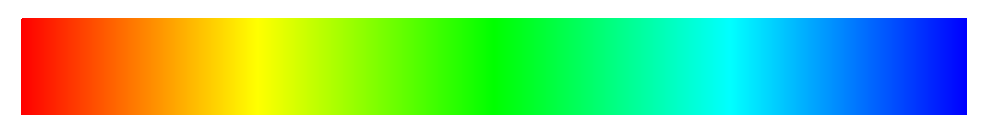
\includegraphics[width=10cm]{images/part11}

\end{center} \end{figure}
\end{frame}

\begin{frame}[fragile,squeeze]
\frametitle{Кодирование цвета}

Основные цвета в разложении белого света --- красный, оранжевый, желтый, зеленый, голубой, синий и фиолетовый образуют так называемый видимый свет видимый свет, тот свет, который воспринимается человеческм глазом. Каждый из цветов характеризуется длиной своей волны.

\end{frame}


\subsection{Цветовые модели}
\begin{frame}[fragile,squeeze]
\frametitle{Аддитивная цветовая модель RGB}
\textit{Аддитивный цвет}\index{цветовая модель!RGB} получается при соединении лучей света разных цветов. В этой системе отсутствие всех цветов представляет собой \textit{черный} цвет, а присутствие всех цветов --- \textit{белый}. Система аддитивных цветов работает с излучаемым цветом работает с излучаемым светом, например от монитора компьютера, экрана телевизора.

Эта модель используется для описания цветов, которые получаются с помощью устройств, основанных на принципе излучения. В качестве основных цветов выбран красный (Red), зеленый (Green) и синий (Blue). Иные цвета и оттенки получаются смешиванием определенного количества указанных основных цветов.
\end{frame}
\begin{frame}[fragile,squeeze]
\frametitle{Аддитивная цветовая модель RGB}

\begin{figure}[htbp] \begin{center}
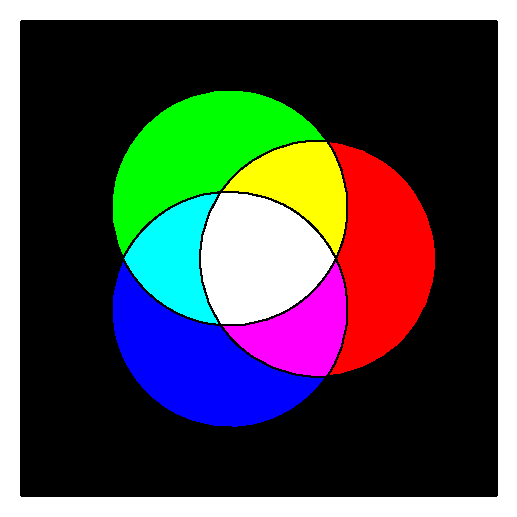
\includegraphics{images/part14}
\caption{Аддитивная модель RGB} 
\end{center} \end{figure}
\end{frame}



\begin{frame}[fragile,squeeze]
\frametitle{Субстрактивная цветовая модель CMYK}

В системе \textit{субстрактивных}\index{цветовая модель!CMYK} цветов происходит обратный процесс: цвет получается вычитанием других цветов из луча света. В этой модели белый цвет появляется в результате отсутствия всех цветов, тогда как их присутствие дает черный цвет. Система субстрактивных цветов работает с отраженным светом, например от листа бумаги. Белая бумага отражает все цвета, окрашенная - некоторые поглощает, остальные отражает.

Название данной модели CMYK составлено из названий основных субтрактивных цветов - голубого (Cyan), пурпурного (Magenta) и желтого (Yellow).
\end{frame}
\begin{frame}[fragile,squeeze]
\frametitle{Субстрактивная цветовая модель CMYK}

\begin{figure}[htbp] \begin{center}
\includegraphics{images/part16}
\end{center} \end{figure}
\end{frame}


\begin{frame}[fragile,squeeze]
\frametitle{Кодирование цвета. Палитра}

Для того чтобы компьютер имел возможность работать с цветными изображениями, необходимо представлять цвета в виде чисел - кодировать цвет. 

Способ кодирования зависит от цветовой модели и формата числовых данных в компьютере.

Для модели RGB каждая из компонент может представляться числами, ограниченными некоторым диапазоном --- например, дробными числами от 0 до 1 либо целыми числами от 0 до некоторого максимального значения. 

\end{frame}

\begin{frame}[fragile,squeeze]
\frametitle{Кодирование цвета. Палитра}

В настоящее время достаточно распространенным является формат True Color, в котором каждая компонента представлена в виде байта, что дает 256 градаций для каждой компоненты: R=0...255, G = 0...255, В = 0...255. 

Количество цветов составляет $256\times256\times256 = 16.7$ млн ($2^{24}$).
\end{frame}

\begin{frame}[fragile,squeeze]
\frametitle{Растровые изображения}

Растровая графика описывает объект цветными точками --- пикселями, определенным образом размещенными в координатной сетке.
Изображение описывается положением и цветом всех точек, из которых, как из мозаики, складывается единый объект.
Редактируя растровые объекты, можно менять только точки, а не линии.
Вся площадь изображения разбивается на некоторое число строк и столбцов. В каждой ячейке полученной матрицы находится элемент, называемый \textit{пикселом}\index{пиксель} (от англ. picture element).

\end{frame}

\begin{frame}[fragile,squeeze]
\frametitle{Растровые изображения}

Основной характеристикой такого элемента является его цвет. По существу редактирование растровых изображений сводится к изменению цветов отдельных пикселов. 

Для того, чтобы записать значение цвета в память компьютера, ему ставят в соответствие одно или несколько целых чисел, обычно, в диапазоне от 0 до 255.

Например, для черно-белой фотографии можно использовать схему, в которой черному цвету соответствует 0, белому - 255, а прочим оттенкам - целые числа внутри этого интервала 
\begin{figure}[htbp] \begin{center}
\includegraphics{images/part17}
\caption{Палитра оттенков серого}
\end{center} \end{figure}
\end{frame}



\begin{frame}[fragile,squeeze]
\frametitle{Растровые изображения}

Рассмотрим процесс преобразования рисунка в цифровую форму на примере. Возьмем черный крест на белом фоне, слева, и попробуем представить запись его компьютерного аналога.
\begin{figure}[htbp] \begin{center}
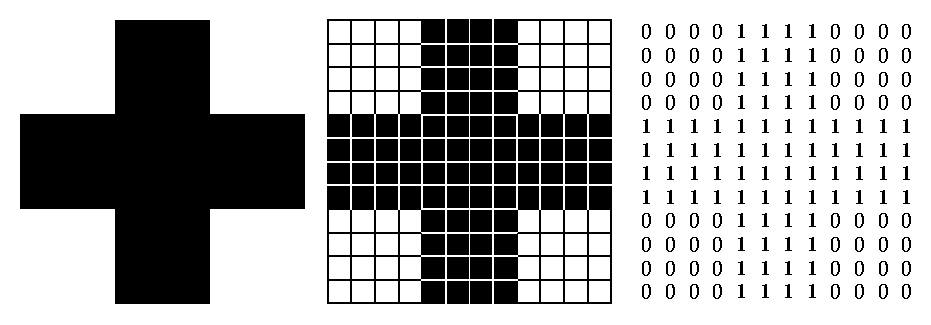
\includegraphics[height=3.5cm]{images/part18}
\end{center} \end{figure}
\end{frame} 

\begin{frame}[fragile,squeeze]
\frametitle{Растровые изображения}

\begin{figure}[htbp] \begin{center}
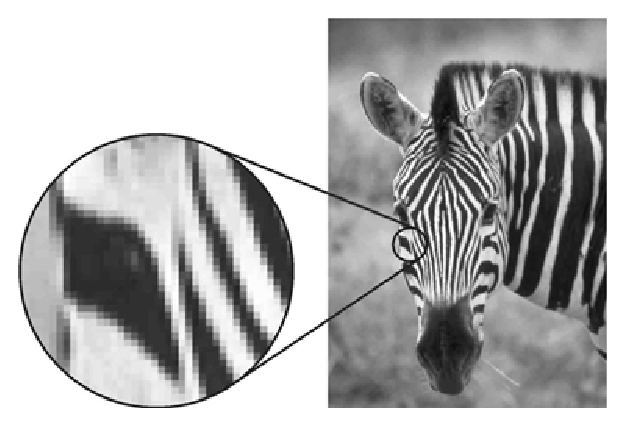
\includegraphics{images/raster}
\end{center} \end{figure}
\end{frame}

\begin{frame}[fragile,squeeze]
\frametitle{Кодирование изображений}
\framesubtitle{Количество информации}

Информационный объем растрового изображения вычисляется по формуле:
$$ V=i\cdot H\cdot W,$$
где $i$-количество бит используемое для хранения цвета 1 пиксела, $H$ --- высота изображения, $W$ --- ширина изображения.

Для хранения цвета используется алфавитный подход и равномерное кодирование.
Для вычисления количества бит, приходящихся на 1 пиксель необходимо использовать формулу Хартли.
\end{frame}

\begin{frame}[fragile,squeeze]
\frametitle{Кодирование изображений}
\framesubtitle{Пример}

\textbf{Задача.} Какой объём памяти в килобайтах необходимо выделить под хранение растрового изображения размером $256\cdot512$ пикселей, если в палитре изображения 16 цветов?
 \\ \pause
\textbf{Решение.} Определяем количество бит, необходимых для  коди-рования одного пикселя: 
$16 = 2^4$, следовательно $i=4$ бита.
Информационный объём: 
$$V=4\cdot 2^8 \cdot 2^9=2^{18} бит$$

или 64 Кбайта.

\end{frame}

 \subsection{Кодирование звука}

\begin{frame}[fragile,squeeze]
\frametitle{Аналого-цифровое преобразование}

Процесс аналого-цифрового преобразования (оцифровки) звука заключается в осуществлении замеров амплитуды сигнала с определенным временным шагом и последующей записи полученных значений в числовом виде.

Таким образом, оцифровка звука включает в себя:
\begin{itemize}
\item процесс дискретизации сигнала по времени;
\item процесс квантования по амплитуде.

\end{itemize}

\end{frame}

\begin{frame}[fragile,squeeze]
\frametitle{Аналого-цифровое преобразование}

\textbf{Частота дискретизации} (или частота семплирования, англ. Sample rate) – частота взятия отсчётов непрерывного по времени (аналогового) сигнала при его дискретизации; измеряется в кГц;

\textbf{Квантование} (англ. Quantization, bitrate, разрешение, уровень квантования, глубина дискретизации) – количество бит, необходимых для хранения одного замера (семпла). (битрейт)

В условиях задач встречается как непосредственно глубина дискретизации, так и количество уровней замеров. Тогда по количеству уровней необходимо пересчитать глубину дискретизации.


\end{frame}

\begin{frame}[fragile,squeeze]
\frametitle{Аналого-цифровое преобразование}

\includegraphics[height=7cm]{images/sound.png}

\end{frame}


\begin{frame}[fragile,squeeze]
\frametitle{Кодирование звука}
\framesubtitle{Количество информации}

Информационный объем звукового файла вычисляется по формуле:
$$ V=i\cdot k\cdot F \cdot t,$$
где $i$-количество бит используемое для хранения кванта звука (битрейт)
\\ 
$k$ --- количество канало записи,\\
$F$ --- частота\\
$t$ --- длительность в секундах\\

Для хранения звука используется алфавитный подход и равномерное кодирование.
Для вычисления количества бит, приходящихся на 1 квант звука необходимо использовать формулу Хартли.
\end{frame}

\begin{frame}[fragile,squeeze]
\frametitle{Кодирование звука}
\framesubtitle{Пример}

\textbf{Задача.} Производится одноканальная (моно) звукозапись с частотой дискретизации 48 кГц и 32-битным разрешением. Запись длится 5 минут ($5\cdot 60=300$секунд), её результаты записываются в файл, сжатие данных не производится. Определите приблизительно объем полученного файла в мегабайтах. В ответе укажите ближайшее к объему файла целое число, кратное 5.\\ \pause
\textbf{Решение.} 
$$ V=32 \cdot 1\cdot 48000\cdot 300=2^5\cdot 2^4\cdot 3 \cdot \overbrace{1000}^{8\cdot125} \cdot 3\cdot \overbrace{100}^{4\cdot 25}$$
$$ V=2^{14}\cdot 3^2 \cdot 5^5 бит!$$



\end{frame}
\begin{frame}[fragile,squeeze]
\frametitle{Кодирование звука}
\framesubtitle{Пример}


$V=2^{14}\cdot 3^2 \cdot 5^5$бит! Переведем в мегабайты
$$ V=\frac{2^{14}\cdot 3^2 \cdot 5^5}{2^{23}}=\frac{3^2 \cdot 5^5}{2^{9}}=\frac{9\cdot125 \cdot 25}{512}$$
$$ V=\frac{1125 \cdot 25}{512}=\frac{(2\cdot 512+ 101)\cdot 25}{512}=\frac{50\cdot 512+ 101\cdot 25}{512}$$
$$ V=50+\frac{101\cdot 25}{512}=50+\frac{2525}{512}=50+\frac{4\cdot 512 +477}{512}=54+\frac{477}{512}$$
Ответ 55 Мб.



\end{frame}
